\documentclass[tikz,border=10pt]{standalone}
\usepackage{pgfplots}
\pgfplotsset{compat=newest}
% \pgfplotsset{compat=1.18}
\usepackage[american]{circuitikz}
\usepackage{cmbright}

\definecolor{myred}{RGB}{170,0,0}
\definecolor{myblue}{RGB}{0,0,220}
\definecolor{mygreen}{RGB}{0,150,0}
\definecolor{myorange}{RGB}{255,127,0}
\definecolor{mybrown}{RGB}{150,75,0}

\ctikzset{bipoles/resistor/height=0.2}
\ctikzset{bipoles/resistor/width=0.5}
\ctikzset{bipoles/capacitor/height=0.4}
\ctikzset{bipoles/capacitor/width=0.15}


\begin{document}

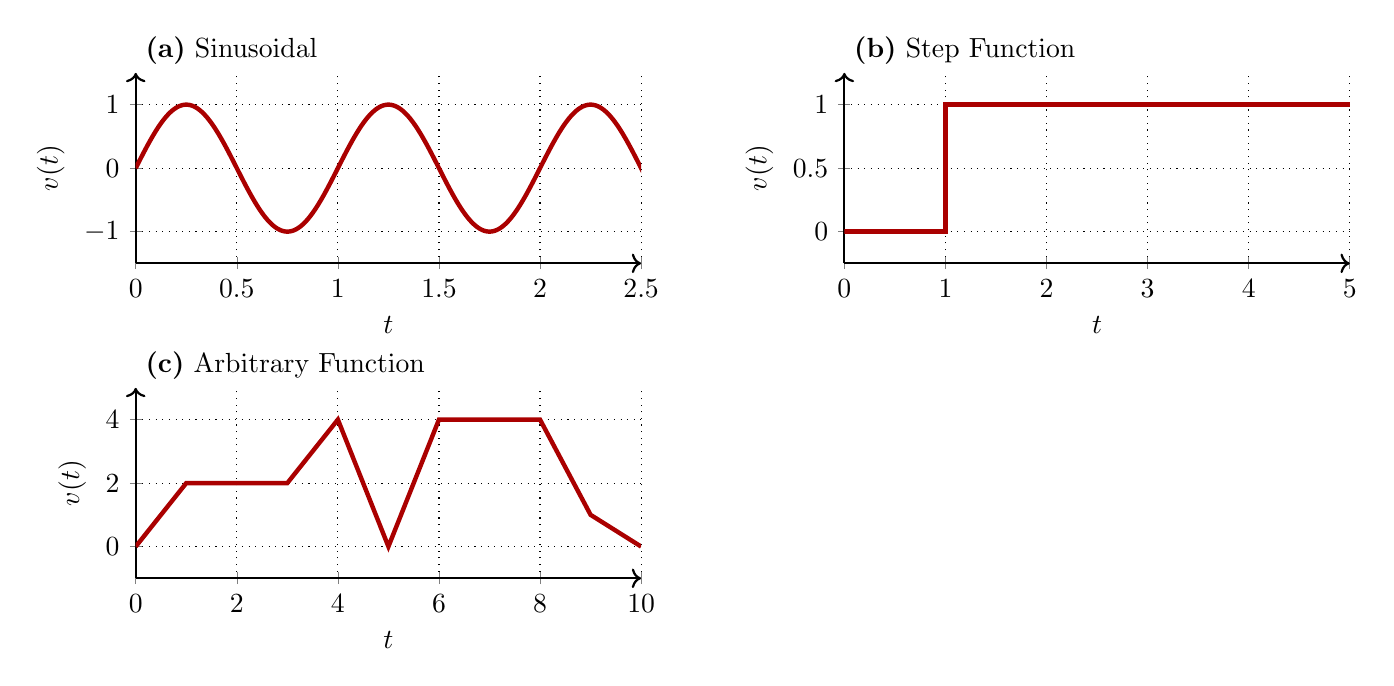
\begin{tikzpicture}

% Plot 1: Sinusoidal
\begin{scope}
    % Display the tile.
    \node[anchor=north west, color=black] at (0, 3) {\textbf{(a)} Sinusoidal};
    \begin{axis}[
        name=plot1,
        width=8cm,
        height=4cm,
        xlabel={$t$},
        ylabel={$v(t)$},
        xmin=0, xmax=2.5,
        ymin=-1.5, ymax=1.5,
        axis lines=left,
        axis line style={->},
        legend style={
            at={(1.05,1.0)},
            anchor=north west,
            draw=none,
            align=left
        },
        thick,
        samples=1000,
        domain=0:5,
        grid=major,
        major grid style={dotted, black}
    ]
    \addplot[myred, ultra thick, domain=0:5] {sin(360 * x)};
    \end{axis}
\end{scope}

% Plot 2: Step Function
\begin{scope}[xshift=9cm]
    % Display the tile.
    \node[anchor=north west, color=black] at (0, 3) {\textbf{(b)} Step Function};
    \begin{axis}[
        name=plot2,
        % at={(plot1.right of south east)}, anchor=left of south west,
        width=8cm,
        height=4cm,
        xlabel={$t$},
        ylabel={$v(t)$},
        xmin=0, xmax=5,
        ymin=-0.25, ymax=1.25,
        axis lines=left,
        axis line style={->},
        legend style={
            at={(1.05,1.0)},
            anchor=north west,
            draw=none,
            align=left
        },
        thick,
        samples=1000,
        domain=0:5,
        grid=major,
        major grid style={dotted, black}
    ]
    \addplot[myred, ultra thick] coordinates {
        (0, 0)
        (1, 0)
        (1, 1)
        (5, 1)
    };
    \end{axis}
\end{scope}


% Plot 3: Arbitrary Function
\begin{scope}[yshift=-4cm]
    % Display the tile.
    \node[anchor=north west, color=black] at (0, 3) {\textbf{(c)} Arbitrary Function};
    \begin{axis}[
        name=plot2,
        % at={(plot1.right of south east)}, anchor=left of south west,
        width=8cm,
        height=4cm,
        xlabel={$t$},
        ylabel={$v(t)$},
        xmin=0, xmax=10,
        ymin=-1, ymax=5,
        axis lines=left,
        axis line style={->},
        legend style={
            at={(1.05,1.0)},
            anchor=north west,
            draw=none,
            align=left
        },
        thick,
        samples=1000,
        domain=0:5,
        grid=major,
        major grid style={dotted, black}
    ]
    \addplot[myred, ultra thick] coordinates {
        (0, 0)
        (1, 2)
        (3, 2)
        (4, 4)
        (5, 0)
        (6, 4)
        (8, 4)
        (9, 1)
        (10, 0)
    };
    \end{axis}
\end{scope}

\end{tikzpicture}

\end{document}